\section{Introduzione all'image segmentation}
L'\textit{image segmentation} (segmentazione dell'immagine) 
\cite{ImageSegmentation_Gradient,ImageSegmentation_Labeller,ImageSegmentation_Provino,Imagesegmentation_pulapakura}
è una tecnica fondamentale della computer vision che consiste nel dividere un'immagine in 
diversi segmenti o regioni, ognuno dei quali rappresenta una parte specifica dell'immagine. 
Questo processo consente alle macchine di comprendere gli elementi all'interno di un'immagine in modo 
più preciso rispetto a compiti come il rilevamento di oggetti.

% Viene utilizzata per ottenere una rappresentazione più compatta, 
% per estrarre degli oggetti o come strumento per l'analisi delle immagini
% Lo scopo della segmentazione è semplificare e/o cambiare la 
% rappresentazione delle immagini in qualcosa che è più significativo e facile da analizzare.

La segmentazione è di solito utilizzata per localizzare oggetti e bordi (linee, curve, ecc.), 
che definiscono le diverse aree di un'immagine. 
Più precisamente, la segmentazione è il processo con il quale si classificano i pixel dell'immagine 
per una qualche proprietà o caratteristica (colore, intensità o texture), assegnando a questi pixel
una \textit{label} (etichetta) di classe.
 
Il risultato di un'immagine segmentata è un insieme di segmenti che, collettivamente, coprono 
l'intera immagine.


\begin{figure}[H]
    \centering
    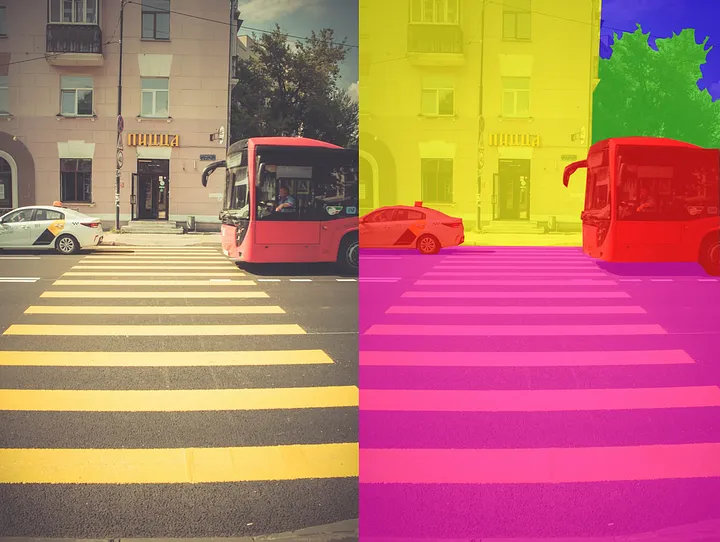
\includegraphics[width=0.70\textwidth]{Immagini/Generiche/esempioImgSegmentation.png}
    \caption{Esempio applicativo dell'image segmentation \cite{Imagesegmentation_pulapakura}.}
\end{figure}

Nella scena di strada sopra, ci sono 5 classi: strada (rosa), veicoli (rosso), edifici (giallo), 
natura (verde), cielo (blu). Ad ogni pixel dell'immagine è stato assegnata una 
di queste classi.

Però a volte, oltre a distinguere le diverse classi, si vuole anche essere in grado di 
distinguere diversi elementi appartenenti 
alla stessa classe. Ad esempio distinguere due auto o alberi. A questo scopo esistono diverse tipologie di segmentazioni, 
ognuna delle quali fornisce dettagli e informazioni differenti.

\subsection{Tipologie di segmentazioni}
Esistono tre tipologie di segmentazione  \cite{ImageSegmentation_Labeller}:
\begin{itemize}
    \item L'\textbf{instance segmentation (segmentazione delle istanze)} consiste nell'identificare e delineare con 
    precisione i singoli oggetti all'interno di un'immagine. A differenza di altri tipi di segmentazione, 
    assegna un'etichetta unica a ogni pixel, fornendo una comprensione dettagliata delle istanze distinte 
    presenti nella scena.

    \item La \textbf{Semantic segmentation (segmentazione semantica)} prevede la classificazione di 
    ogni pixel di un'immagine in categorie predefinite. L'obiettivo è comprendere il contesto generale 
    della scena, assegnando etichette alle regioni in base al loro significato semantico condiviso.

    \item La \textbf{Panoptic segmentation (segmentazione panottica)} rileva anche istanze distinte di 
    ciascun tipo di oggetto. In altre parole, la segmentazione panottica assegna a ogni pixel di un'immagine 
    due etichette: un'etichetta semantica e un ID istanza.
    Gli ID di istanza distinguono le istanze, mentre i pixel con la stessa etichetta sono considerati 
    appartenenti alla stessa classe semantica. A differenza della segmentazione per istanze, la 
    segmentazione panottica assegna un'etichetta distinta a ogni pixel corrispondente a un'istanza 
    individuale per evitare un'interpretazione errata delle informazioni.
\end{itemize}

\begin{figure}[H]
    \centering
    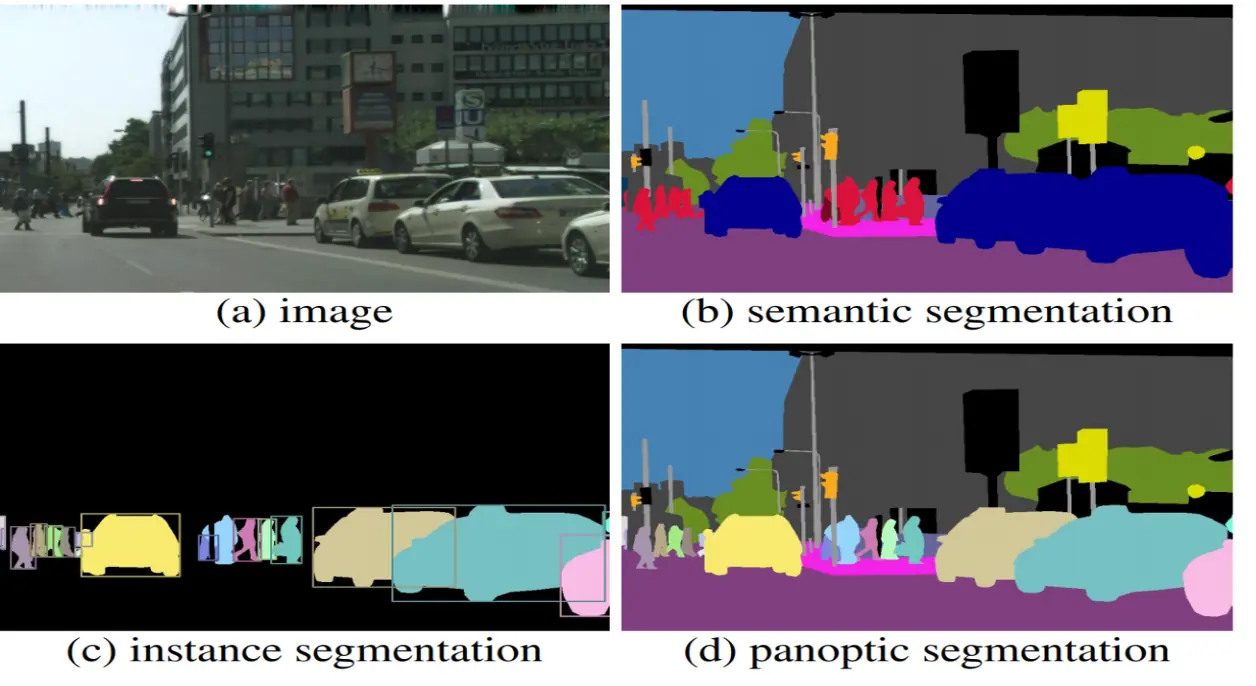
\includegraphics[width=0.8\textwidth]{Immagini/Generiche/semantic_vs_instance_vs_panoptic.png}
    \caption{Rappresentazione applicativa delle diverse tipologie di segmentazioni \cite{ImageSegmentation_Labeller}.}

\end{figure}

Ogni tipo serve ad uno scopo distinto nella computer vision, offrendo vari livelli di granularità 
nell'analisi e nella comprensione del contenuto visivo.
\newpage



